\documentclass[aspectratio=169, 11pt, hyperref={unicode}]{beamer}
\usetheme{Madrid}
\usepackage{pgfplots}
\pgfplotsset{compat=1.17}

\usepackage[czech]{babel}
\usepackage[utf8]{inputenc}
\usepackage[T1]{fontenc}

\usepackage[nodayofweek]{datetime}
\newdate{date}{19}{5}{2023}

\usepackage{graphicx}
\usepackage{subcaption}

\usepackage[euler]{textgreek}
\usepackage[font=footnotesize]{caption}


\title{Branch-line coupler}
\subtitle{B2M17CADA -- Projekt II}
\author{Martin Šimák}
\date{\displaydate{date}}


\definecolor{cvut_navy}{HTML}{0065BD}
\definecolor{cvut_blue}{HTML}{6AADE4}
\definecolor{cvut_gray}{HTML}{156570}

\setbeamercolor{section in toc}{fg=black,bg=white}
\setbeamercolor{alerted text}{fg=cvut_blue}
\setbeamercolor*{palette primary}{bg=cvut_navy,fg=gray!20!white}
\setbeamercolor*{palette secondary}{bg=cvut_blue,fg=white}
\setbeamercolor*{palette tertiary}{parent=palette primary}
\setbeamercolor*{palette quaternary}{fg=green,bg=gray!5!white}

\setbeamercolor*{sidebar}{fg=cvut_navy,bg=gray!15!white}


\setbeamercolor{titlelike}{parent=palette primary}
\setbeamercolor{frametitle}{parent=palette primary}

\setbeamercolor*{separation line}{}
\setbeamercolor*{fine separation line}{}

\setbeamertemplate{navigation symbols}{} 

\setbeamercolor{itemize item}{fg=cvut_blue}
\setbeamercolor{itemize subitem}{fg=cvut_blue}
\setbeamercolor{itemize subsubitem}{fg=cvut_blue}
\setbeamercolor{section number projected}{bg=cvut_navy}
\setbeamercolor{caption name}{fg=cvut_blue}

\setbeamertemplate{itemize item}[circle]
\setbeamertemplate{itemize subitem}[circle]
\setbeamertemplate{itemize subsubitem}[circle]
\setbeamertemplate{caption}[numbered]


\begin{document}

\logo{
\includegraphics[height=1cm]{src/symbol_cvut_plna_samostatna_verze.pdf}}

\begin{frame}
	\titlepage
\end{frame}

\begin{frame}
    \frametitle{Obsah}
    \tableofcontents
\end{frame}

\section{Zadání}
\begin{frame}
\frametitle{Zadání}
Vytvořte a analyzujte v simulátoru CST Studio Suite SE (studentská verze) model vybraného obvodu se vstupní impedancí blízkou $Z_0 = 50\ \Omega$. Redukujte složitost modelu tak, aby měl model maximálně 100 000 buněk mřížky, což limit SE verze pro spuštění řešiče v časové oblasti. Toho lze dosáhnout použitím elektrických, resp. magnetických, stěn, snížením počtu buněk na vlnovou délku, úpravou lokální hustoty mříže, použitím PEC, bezeztrátových materiálů aj.

\textbf{Vybraný obvod:} branch-line coupler, 12,8~GHz
\end{frame}

\begin{frame}
\frametitle{Zadání - úkoly}
Vypočtěte a znázorněte relevantní veličiny: impedanční parametry, rozložení intenzit elektrického a magnetického pole ve vhodných řezech, proudovou hustotu na vodivých částech subkomponenty a tok Poyntigova vektoru, tj. výkonové hustoty. Popište odlišnost frekvenčních průběhů rozptylových a impedančních parametrů (popř. i jiných) pro různou:
\begin{enumerate}
    \item hustotu výpočetní mřížky (počet buněk na vlnovou délku);
    \item hustotu mřížky v oblasti komponent a okolí jejich hran;
    \item zbytkovou hodnotu energie pole ve výpočetní oblasti pro ukončení výpočtu.
\end{enumerate}
\end{frame}

\section{Návrh obvodu v AWR Microwave Office}
\begin{frame}{Návrh obvodu v AWR Microwave Office}
    K výpočtu geometrických parametrů struktury bylo využito softwaru AWR Microwave Office, jehož součástí je podprogram TX-Line. Právě tento podprogram umožňuje výpočet impedancí a ostatních charakteristik běžných přenosových vedení včetně mikropáskové struktury, která je předmětem tohoto projektu. Pro srovnání s výsledkem z programu CST jsou na následujících slidech kromě daného obvodu grafy frekvenční závislosti S-parametrů.
\end{frame}
\begin{frame}{AWR -- Obvod}
	\begin{figure}[!ht]
		\centering
		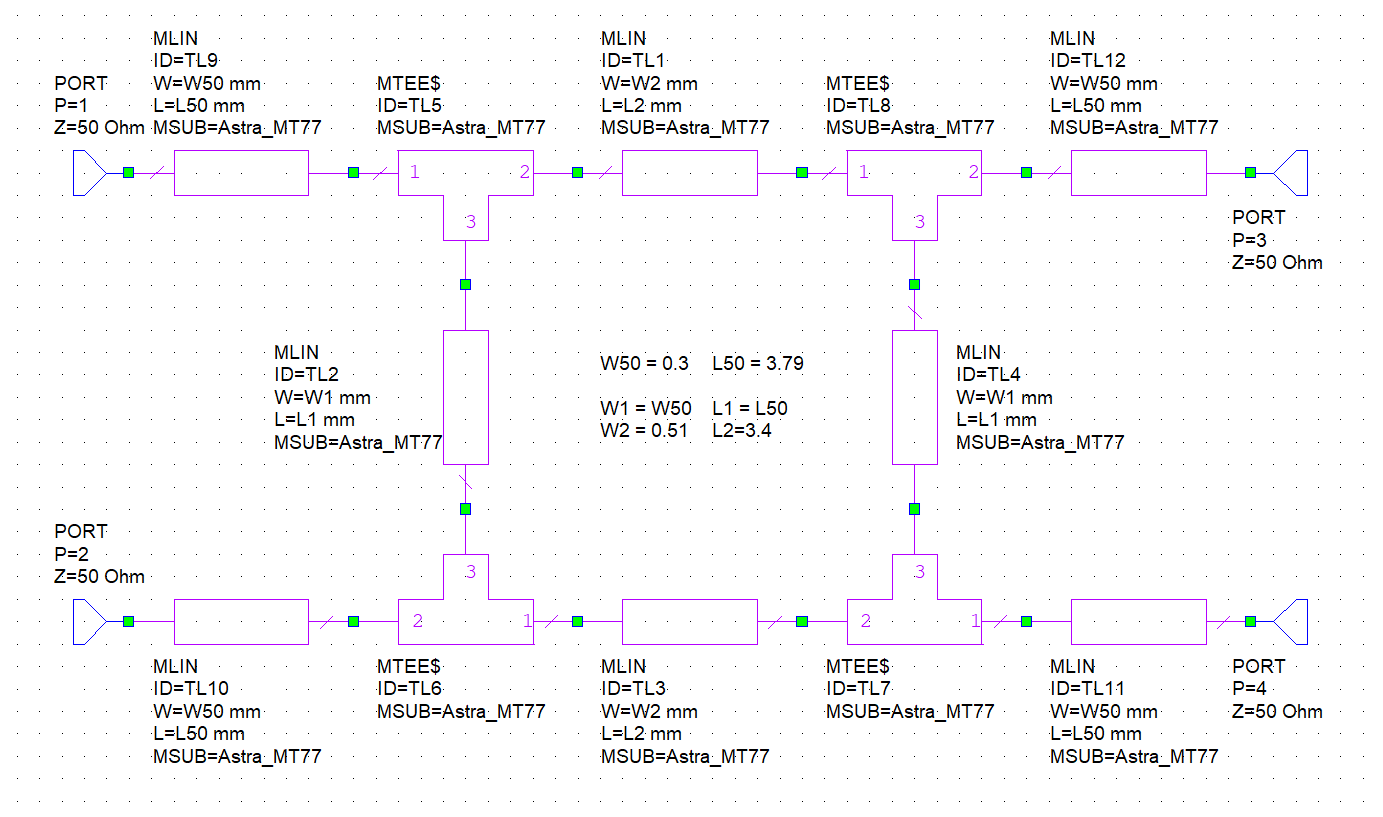
\includegraphics[width=.7\textwidth]{src/AWR_circuit.png}
	\end{figure}
\end{frame}
\begin{frame}{AWR -- S-parametry}
	\begin{figure}[!ht]
		\centering
		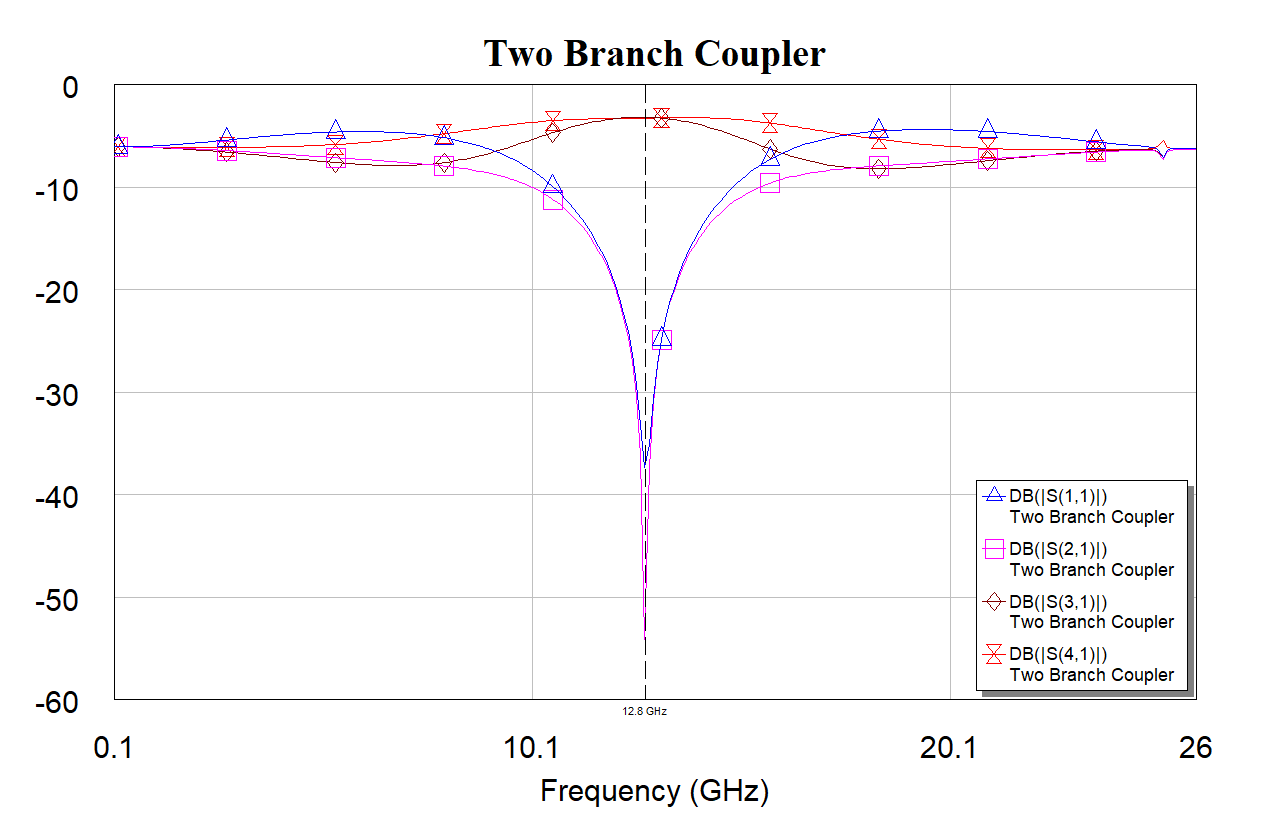
\includegraphics[width=.7\textwidth]{src/AWR_S-parameters.png}
	\end{figure}
\end{frame}
\begin{frame}{AWR -- S-parametry (fáze)}
	\begin{figure}[!ht]
		\centering
		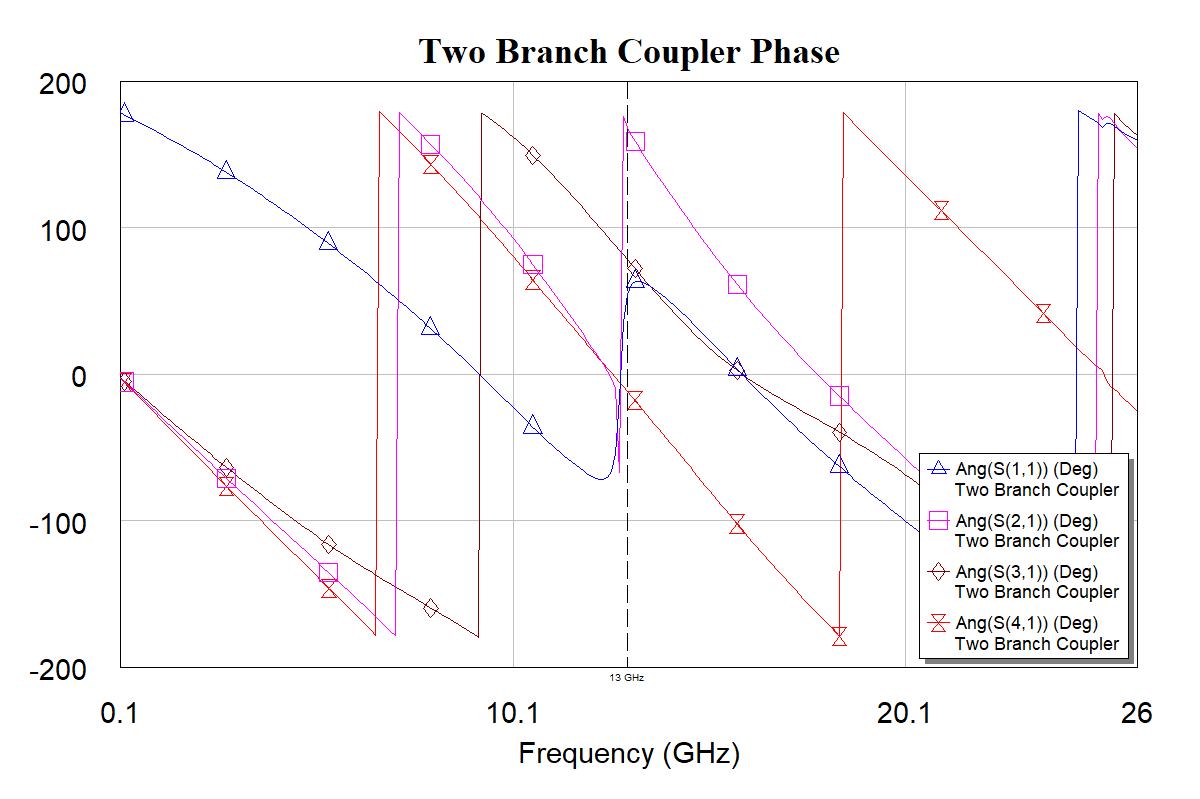
\includegraphics[width=.7\textwidth]{src/AWR_S-parameters_phase.png}
	\end{figure}
\end{frame}

\section{Návrh mikrovlnného obvodu v CST Studio Suite SE}
\begin{frame}{CST -- Izometrický pohled na 3D model obvodu}
	\begin{figure}[!ht]
		\centering
		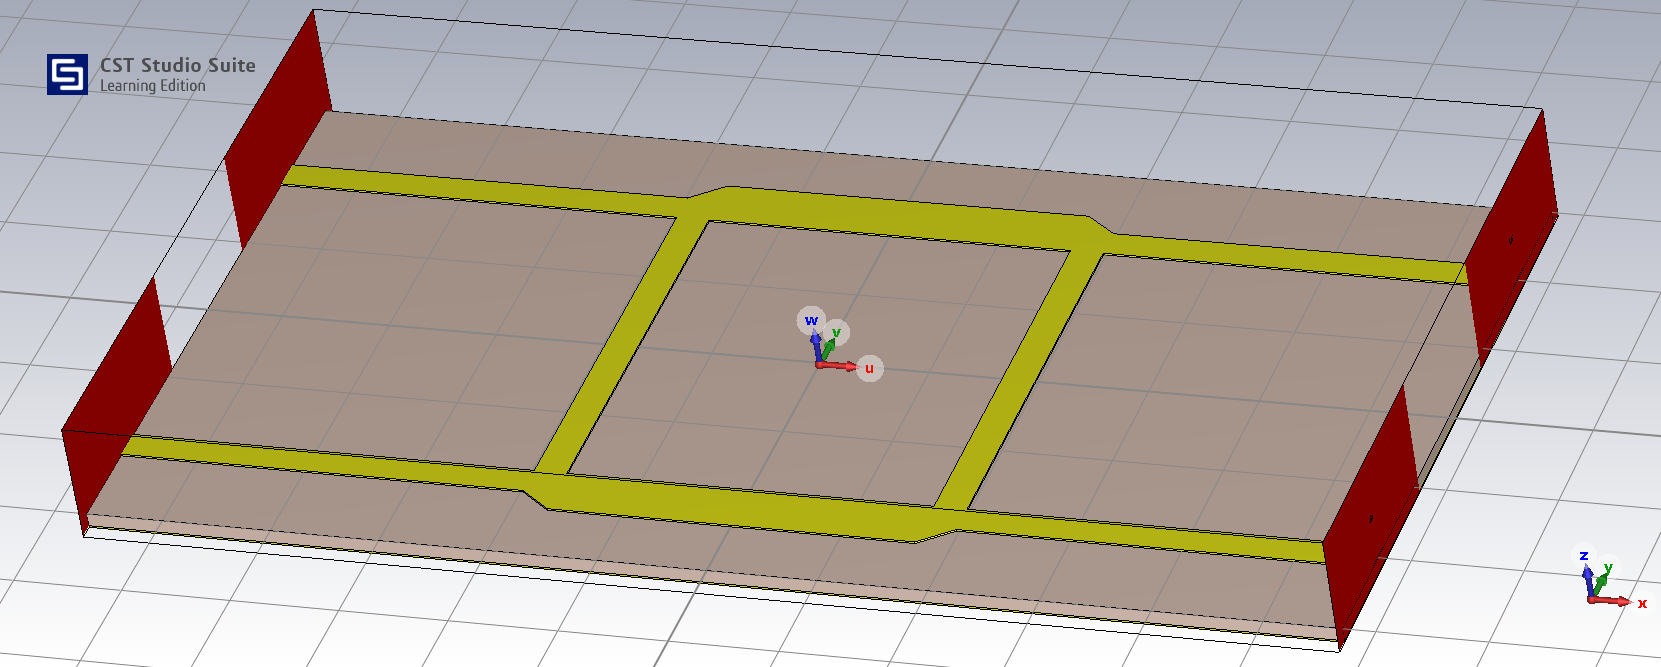
\includegraphics[width=.8\textwidth]{src/CST_3D-isometric.png}
	\end{figure}
\end{frame}

\subsection{Rozložení polí}
\begin{frame}{CST -- Elektrické pole}
	\begin{figure}[!ht]
		\centering
		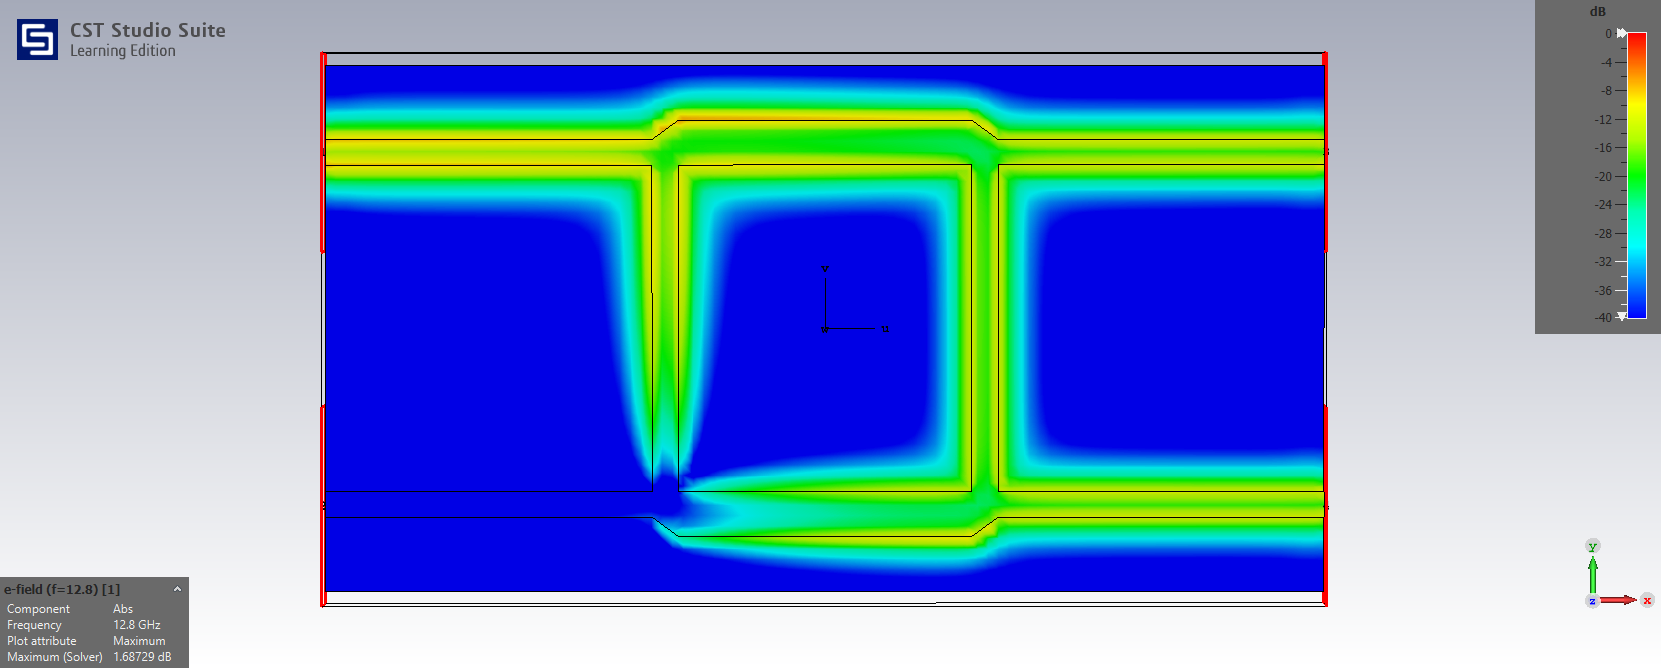
\includegraphics[width=.8\textwidth]{src/CST_E-field_f12-8.png}
	\end{figure}
\end{frame}
\begin{frame}{CST -- Magnetické pole}
	\begin{figure}[!ht]
		\centering
		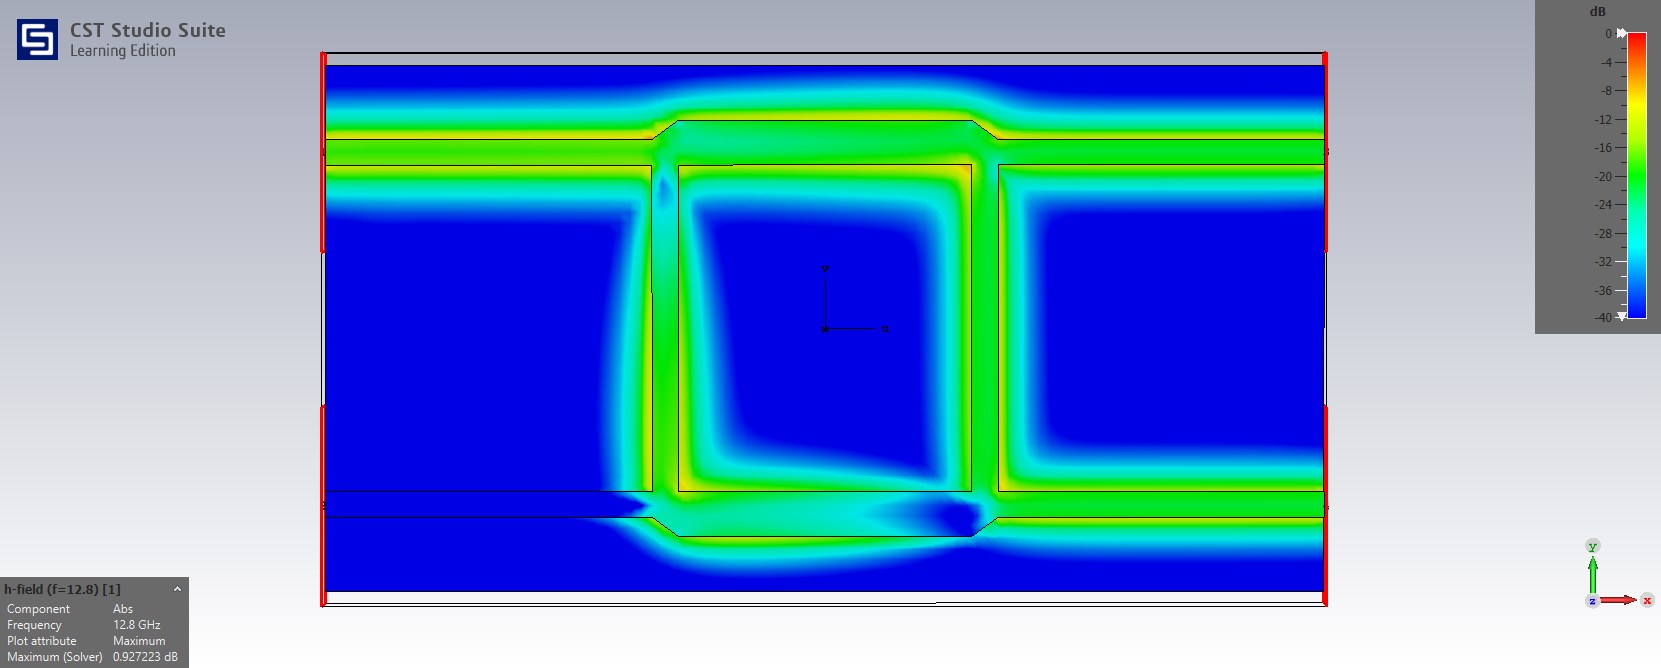
\includegraphics[width=.8\textwidth]{src/CST_H-field_f12-8.png}
	\end{figure}
\end{frame}
\begin{frame}{CST -- Proudová hustota}
	\begin{figure}[!ht]
		\centering
		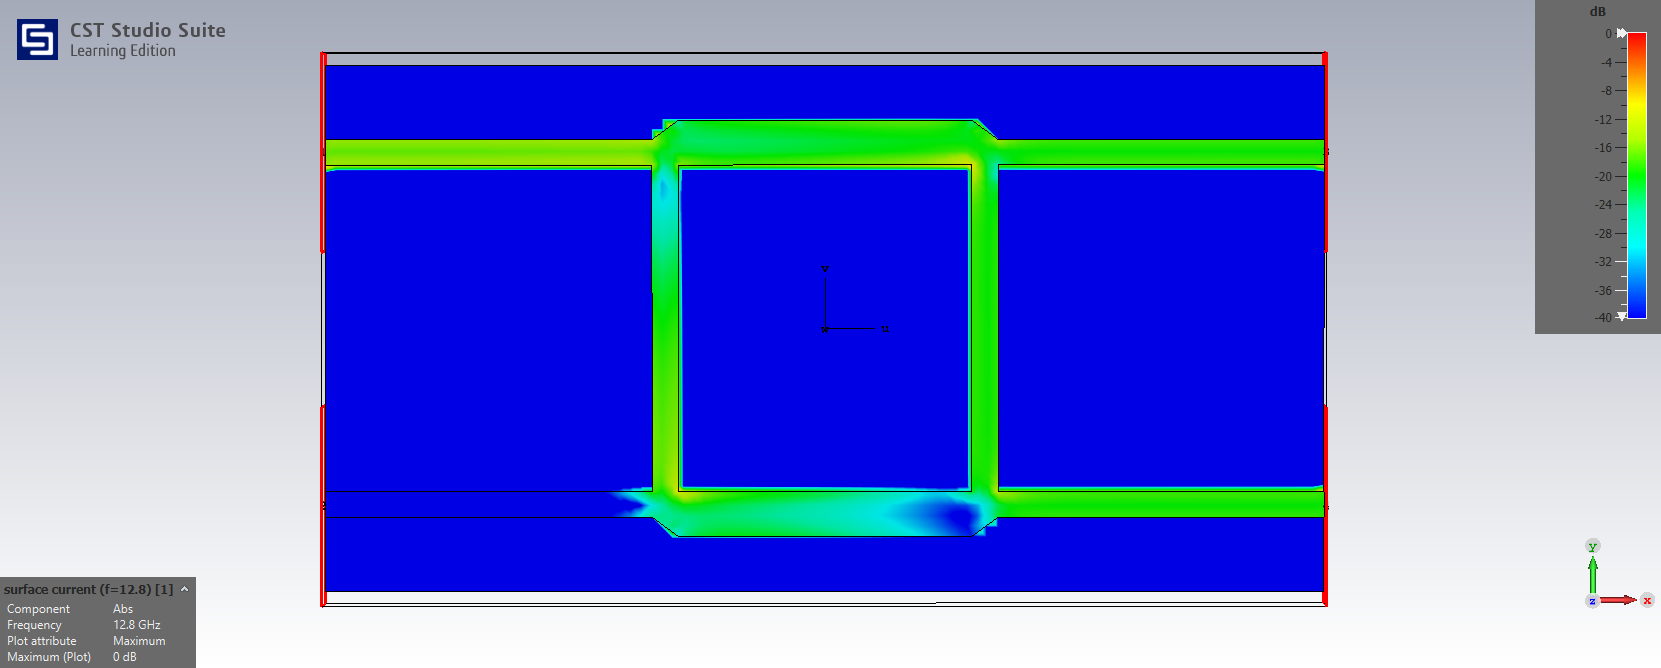
\includegraphics[width=.8\textwidth]{src/CST_J-current_f12-8.png}
	\end{figure}
\end{frame}
\begin{frame}{CST -- Poyntingův vektor (výkonový tok)}
	\begin{figure}[!ht]
		\centering
		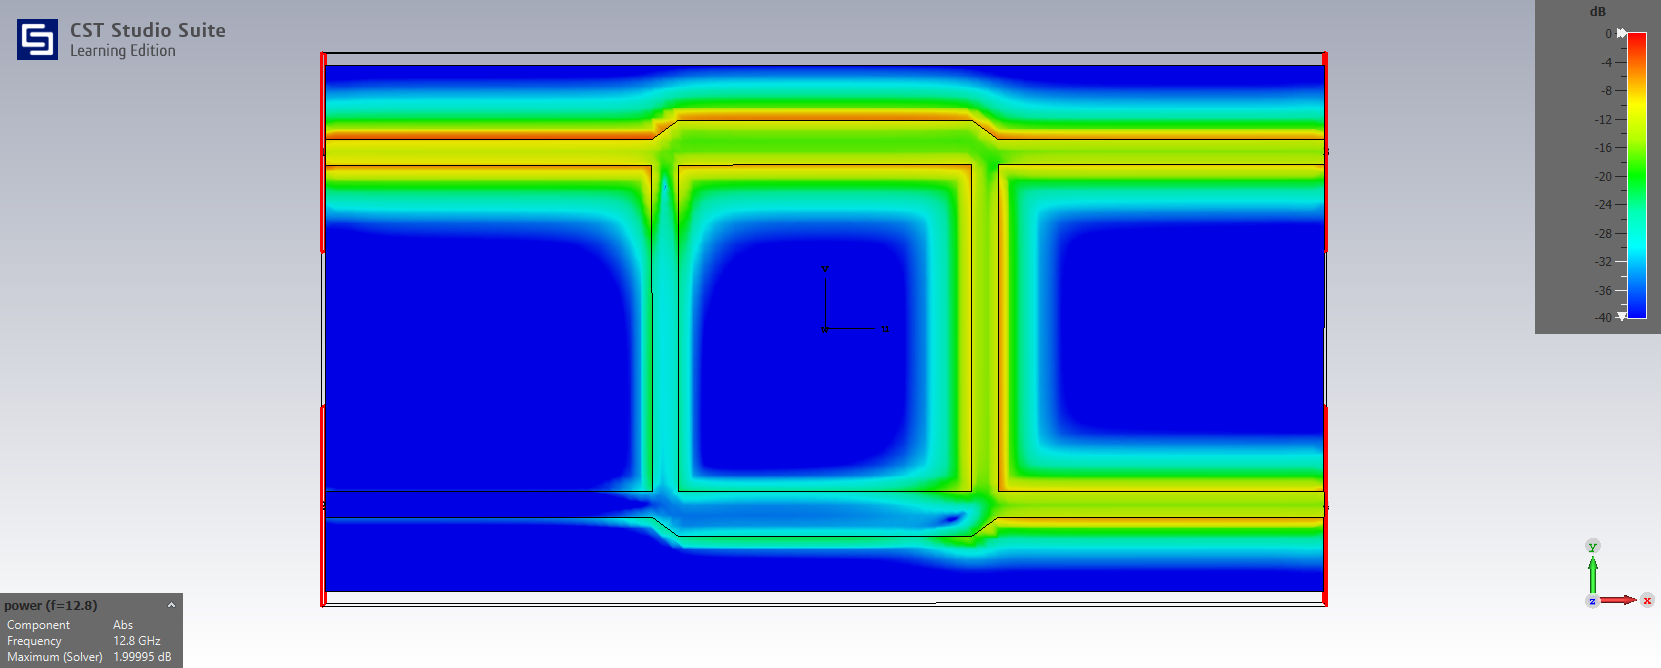
\includegraphics[width=.8\textwidth]{src/CST_power_f12-8.png}
	\end{figure}
\end{frame}

\subsection{S-parametry}
\begin{frame}
    Na následujících slidech je možné nahlédnout na frekvenční průběhy S-parametrů modelované struktury. Parametry výpočtu:
    \begin{itemize}
        \item Acc \dots přesnost výpočtu v podobě zbytkové energie pole ve výpočetní oblasti,
        \item CpW \dots \emph{cells per wavelength}, neboli počet buněk na vlnovou délku, coby globální hustota výpočetní mřížky,
        \item RAE \dots \emph{refinement around edge}, neboli zjemnění kolem hran, coby lokální zjemnění výpočetní mříže v problematických oblastech v blízkosti komponent.
    \end{itemize}
    Průběhy na následujících slidech jsou vykresleny pro hodnoty těchto parametrů, které považuji za dostatečně ilustrativní z hlediska jejich dopadu na výsledek.
\end{frame}
\begin{frame}{CST -- S-parametry pro $\{\text{Acc} = -40\ \text{dB}, \text{CpW} = 10, \text{RAE} = 6\}$}
	\begin{figure}[!ht]
		\centering
		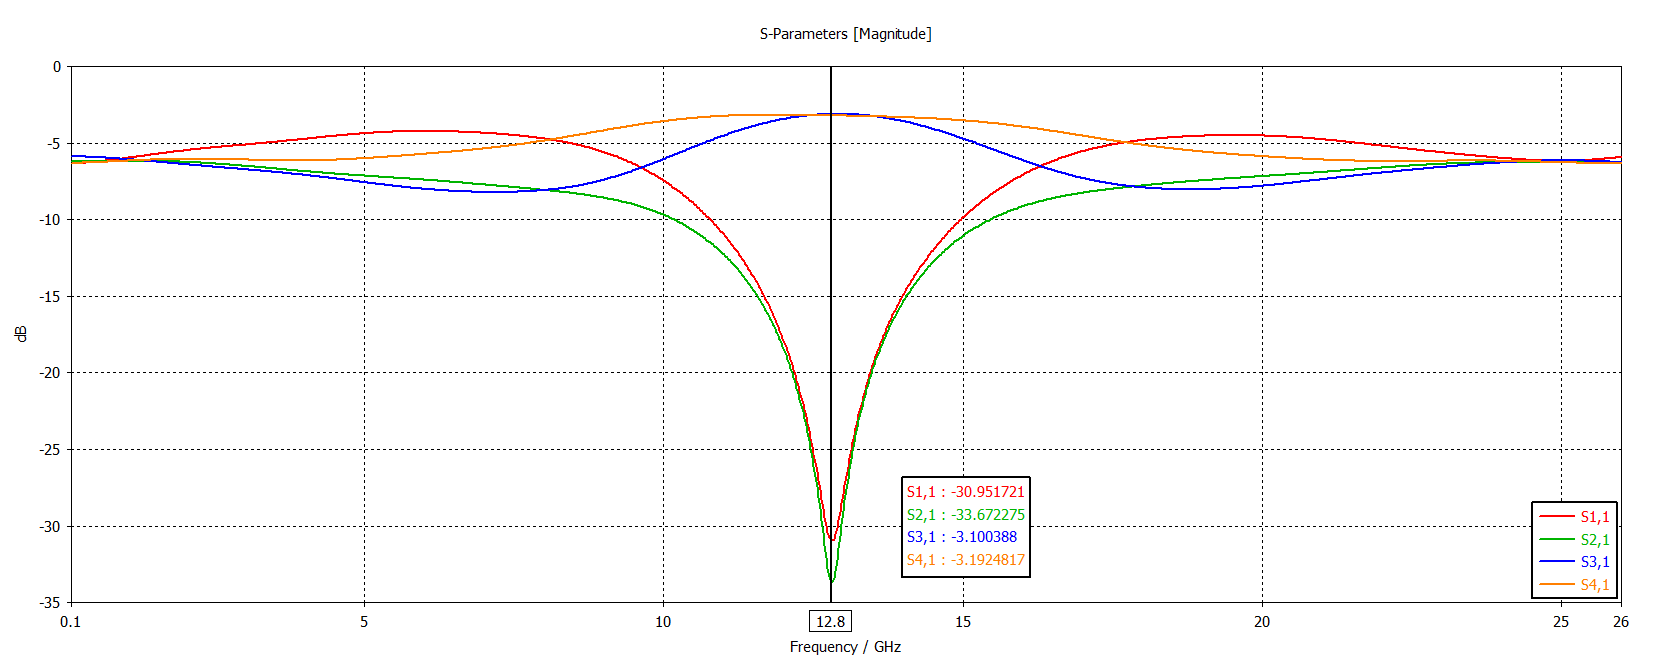
\includegraphics[width=.8\textwidth]{src/CST_S-Parameters_40dB_10-cpw_6-cntm.png}
	\end{figure}
\end{frame}
\begin{frame}{CST -- S-parametry (fáze) pro $\{\text{Acc} = -40\ \text{dB}, \text{CpW} = 10, \text{RAE} = 6\}$}
	\begin{figure}[!ht]
		\centering
		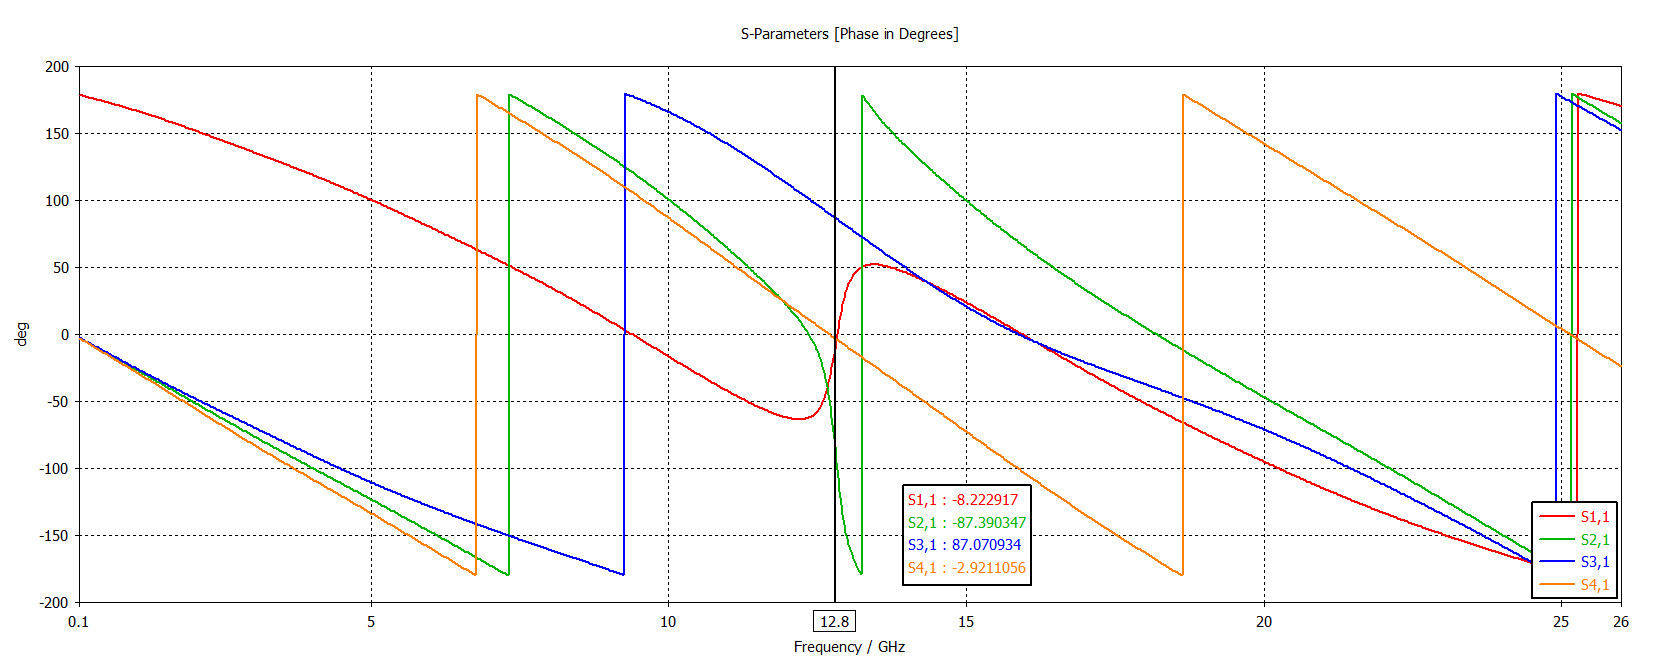
\includegraphics[width=.8\textwidth]{src/CST_S-Parameters_phase_40dB_10-cpw_6-cntm.png}
	\end{figure}
\end{frame}
\begin{frame}{CST -- S-parametry pro $\{\text{Acc} = -30\ \text{dB}, \text{CpW} = 10, \text{RAE} = 6\}$}
	\begin{figure}[!ht]
		\centering
		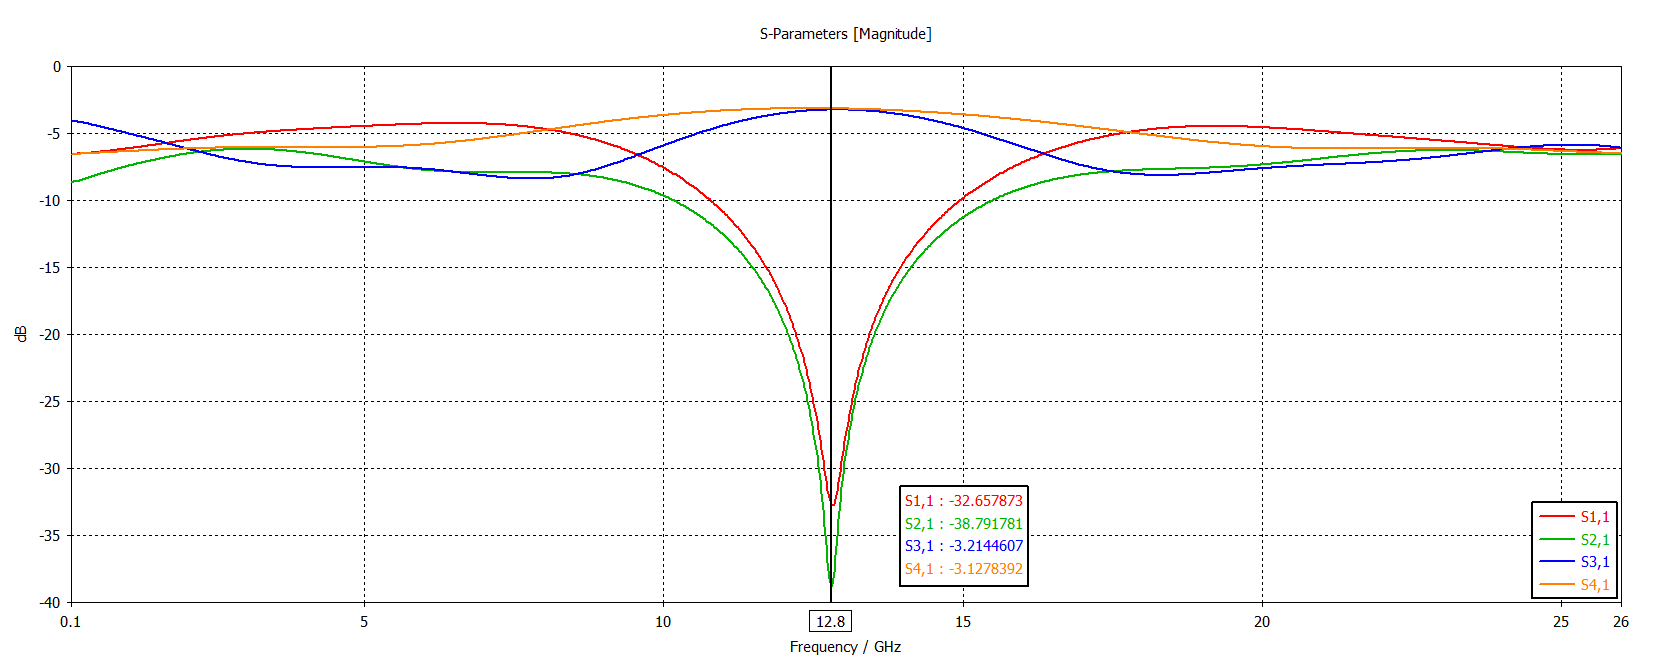
\includegraphics[width=.8\textwidth]{src/CST_S-Parameters_30dB_10-cpw_6-cntm.png}
	\end{figure}
\end{frame}
\begin{frame}{CST -- S-parametry (fáze) pro $\{\text{Acc} = -30\ \text{dB}, \text{CpW} = 10, \text{RAE} = 6\}$}
	\begin{figure}[!ht]
		\centering
		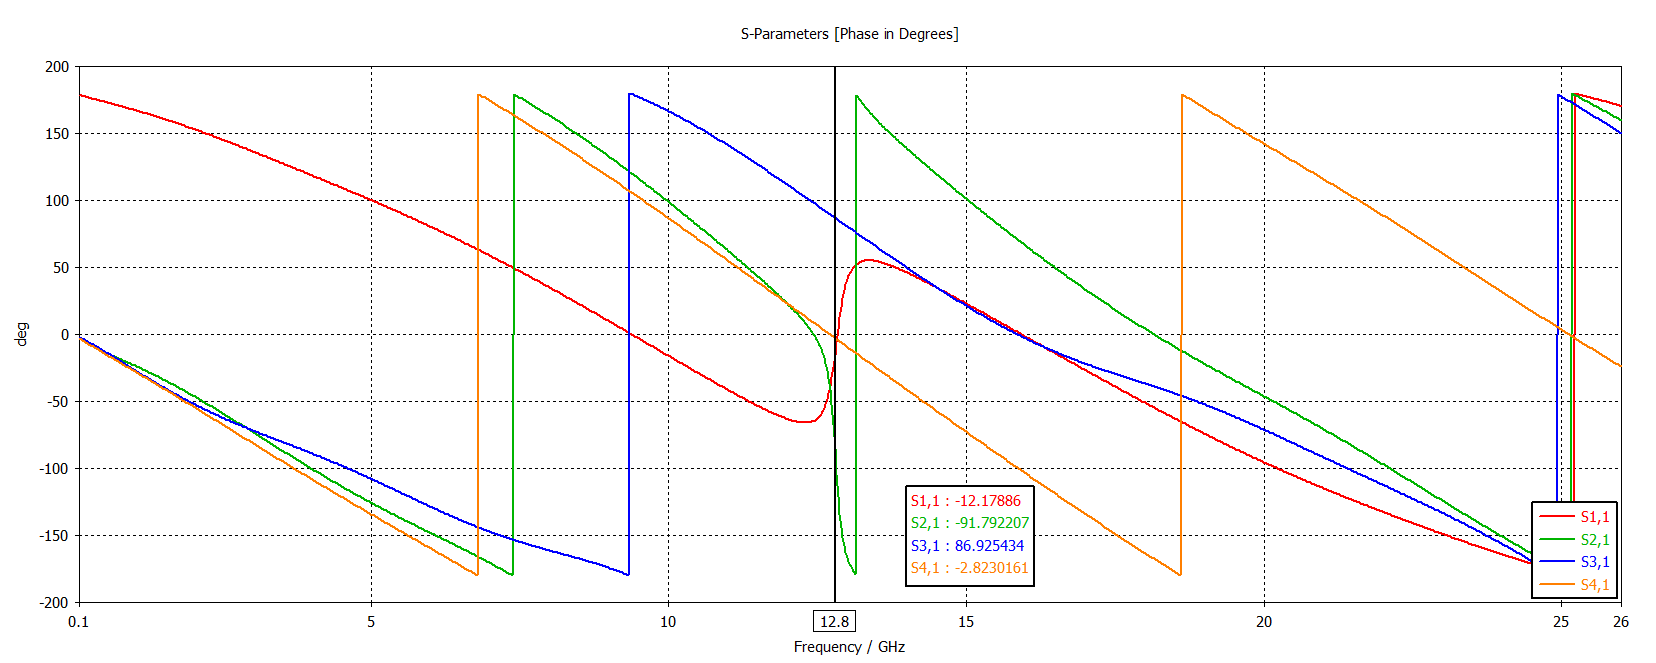
\includegraphics[width=.8\textwidth]{src/CST_S-Parameters_phase_30dB_10-cpw_6-cntm.png}
	\end{figure}
\end{frame}
\begin{frame}{CST -- S-parametry pro $\{\text{Acc} = -20\ \text{dB}, \text{CpW} = 10, \text{RAE} = 6\}$}
	\begin{figure}[!ht]
		\centering
		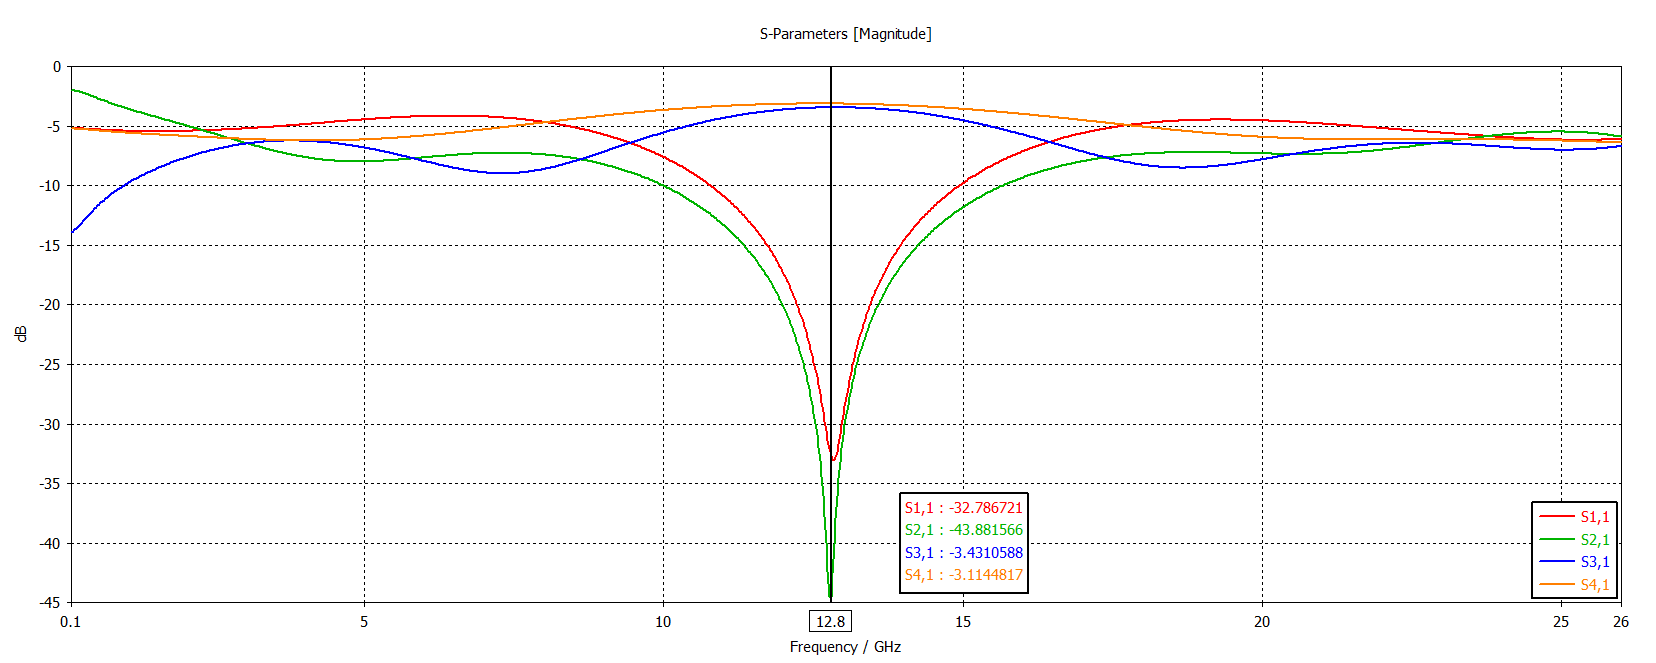
\includegraphics[width=.8\textwidth]{src/CST_S-Parameters_20dB_10-cpw_6-cntm.png}
	\end{figure}
\end{frame}
\begin{frame}{CST -- S-parametry (fáze) pro $\{\text{Acc} = -20\ \text{dB}, \text{CpW} = 10, \text{RAE} = 6\}$}
	\begin{figure}[!ht]
		\centering
		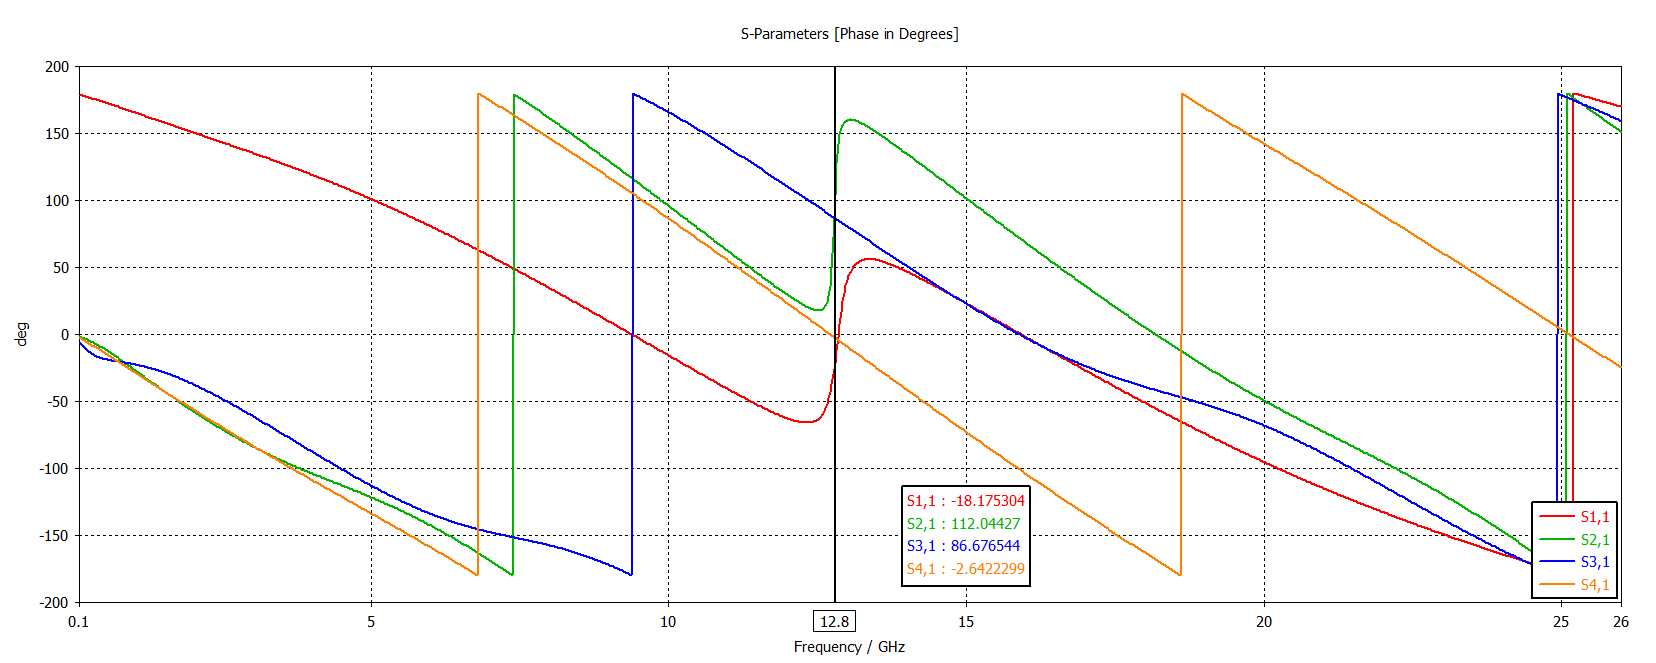
\includegraphics[width=.8\textwidth]{src/CST_S-Parameters_phase_20dB_10-cpw_6-cntm.png}
	\end{figure}
\end{frame}
\begin{frame}{CST -- S-parametry pro $\{\text{Acc} = -40\ \text{dB}, \text{CpW} = 4, \text{RAE} = 6\}$}
	\begin{figure}[!ht]
		\centering
		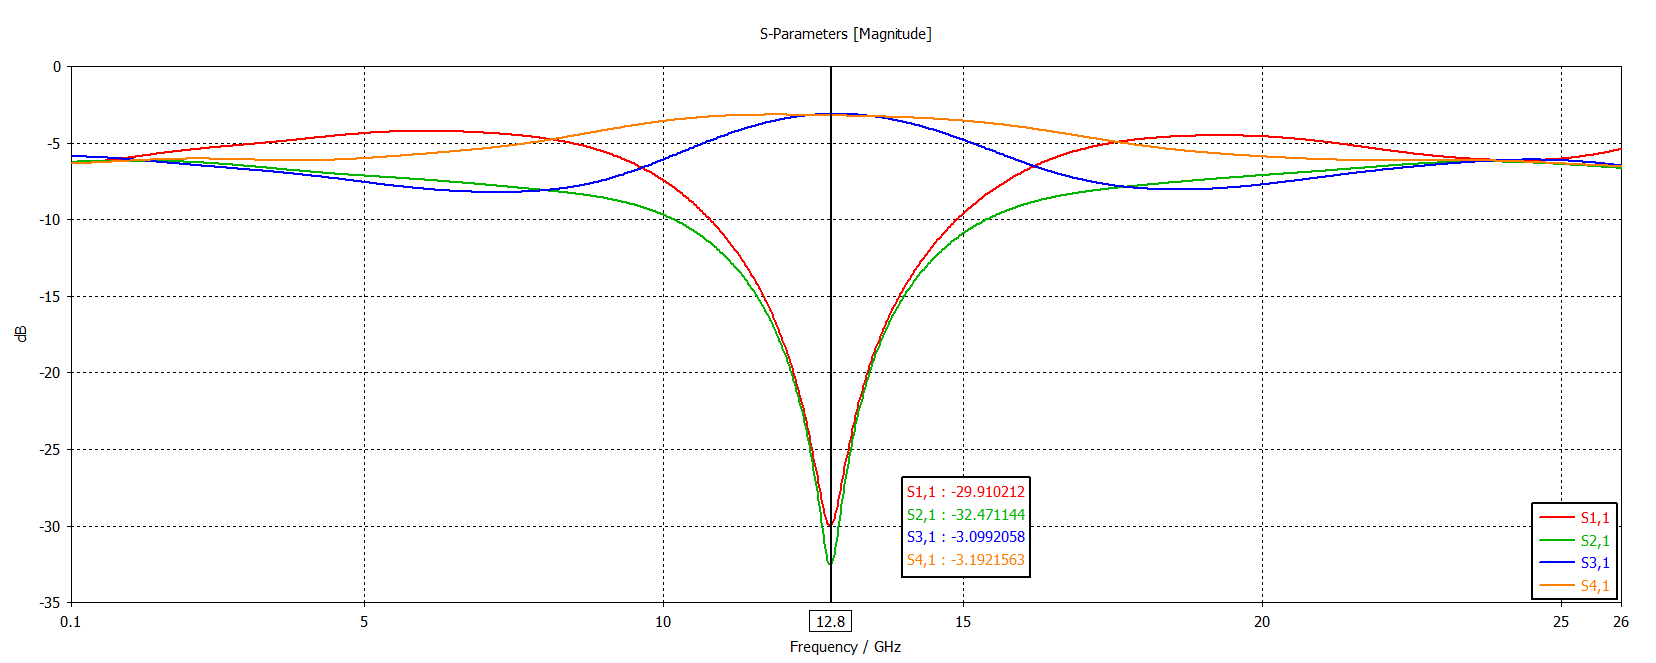
\includegraphics[width=.8\textwidth]{src/CST_S-Parameters_40dB_4-cpw_6-cntm.png}
	\end{figure}
\end{frame}
\begin{frame}{CST -- S-parametry (fáze) pro $\{\text{Acc} = -40\ \text{dB}, \text{CpW} = 4, \text{RAE} = 6\}$}
	\begin{figure}[!ht]
		\centering
		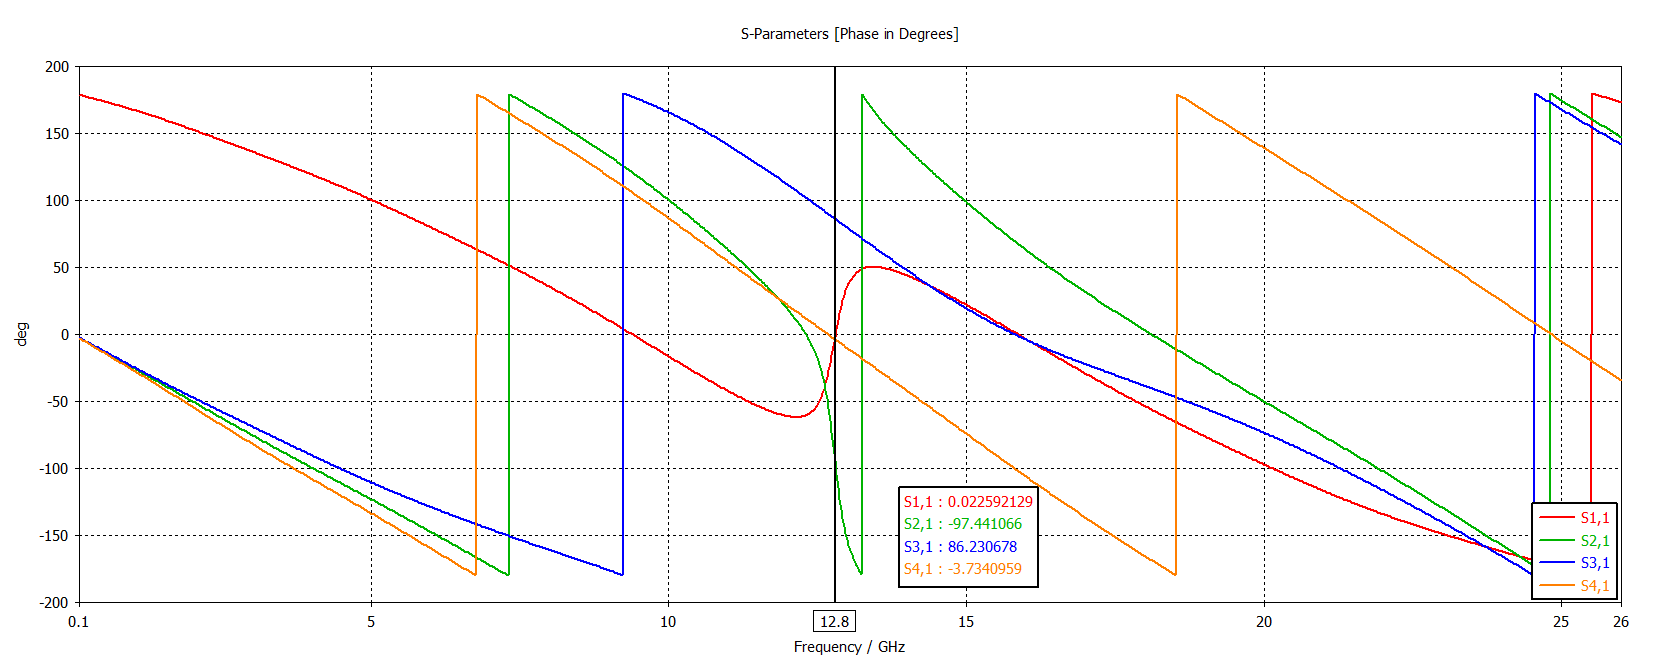
\includegraphics[width=.8\textwidth]{src/CST_S-Parameters_phase_40dB_4-cpw_6-cntm.png}
	\end{figure}
\end{frame}
\begin{frame}{CST -- S-parametry pro $\{\text{Acc} = -40\ \text{dB}, \text{CpW} = 10, \text{RAE} = 1\}$}
	\begin{figure}[!ht]
		\centering
		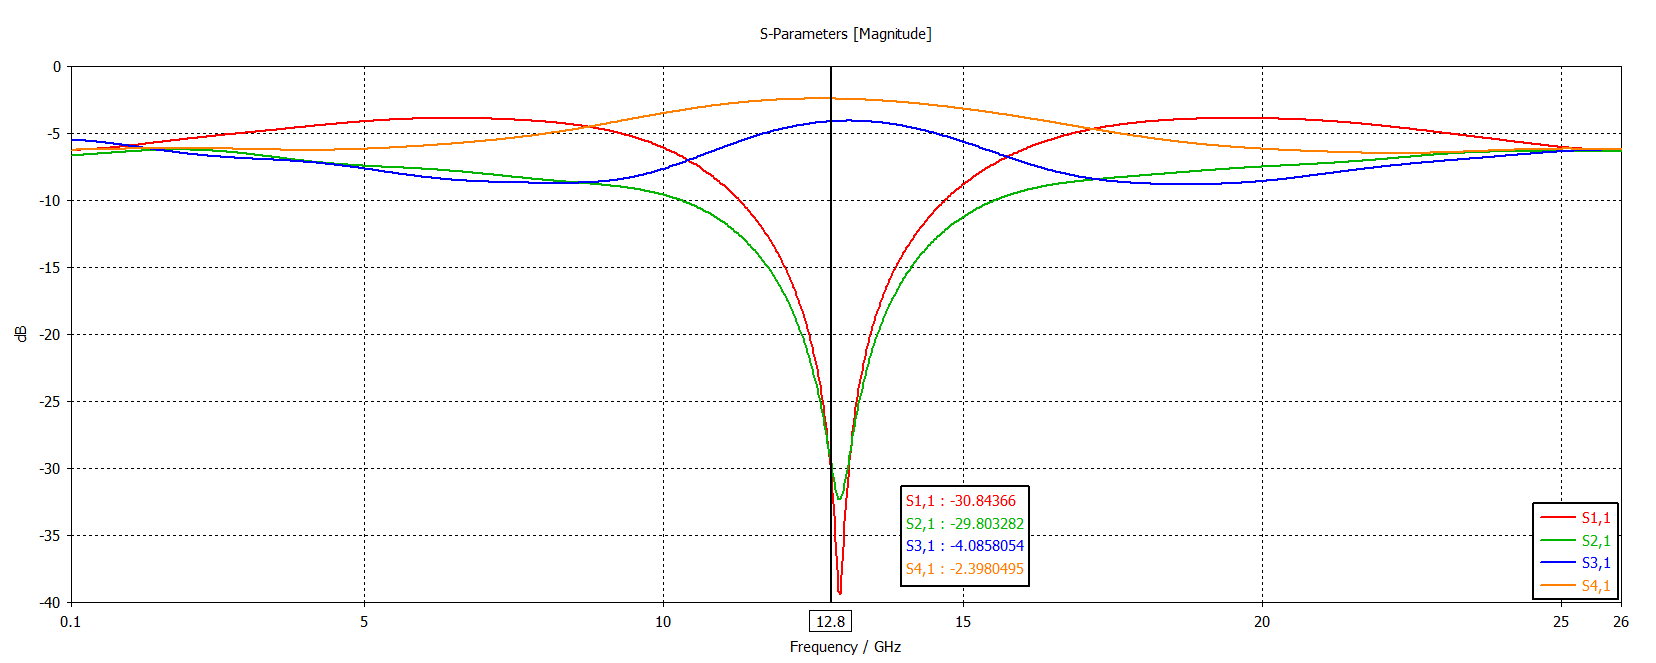
\includegraphics[width=.8\textwidth]{src/CST_S-Parameters_40dB_10-cpw_1-cntm.png}
	\end{figure}
\end{frame}
\begin{frame}{CST -- S-parametry (fáze) pro $\{\text{Acc} = -40\ \text{dB}, \text{CpW} = 10, \text{RAE} = 1\}$}
    \begin{figure}[!ht]
        \centering
        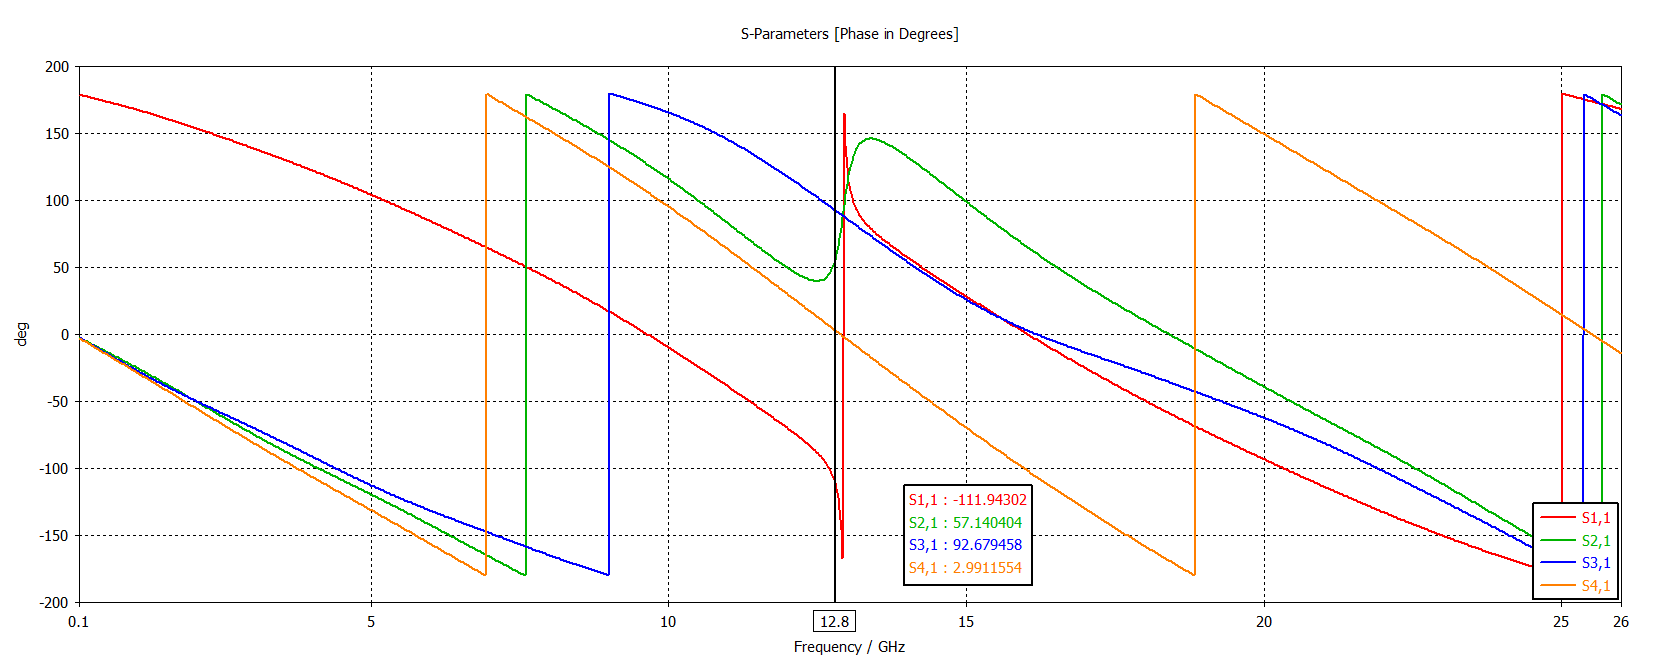
\includegraphics[width=.8\textwidth]{src/CST_S-Parameters_phase_40dB_10-cpw_1-cntm.png}
    \end{figure}
\end{frame}

\subsection{Vstupní impedance}
\begin{frame}{Vstupní impedance}
    Vstupní impedance nebyla změnami hodnot přesnosti výpočtu či hustot výpočetní mřížky příliš zatížena. Všechny vygenerované průběhy jsou konstatní s hodnotou impedance $(50 \pm 0,5)\ \Omega$. Uvádíme tedy pouze jeden průběh pro $\{\text{Acc} = -40\ \text{dB}, \text{CpW} = 10, \text{RAE} = 6\}$.
\end{frame}
\begin{frame}{CST -- Vstupní impedance}
	\begin{figure}[!ht]
		\centering
		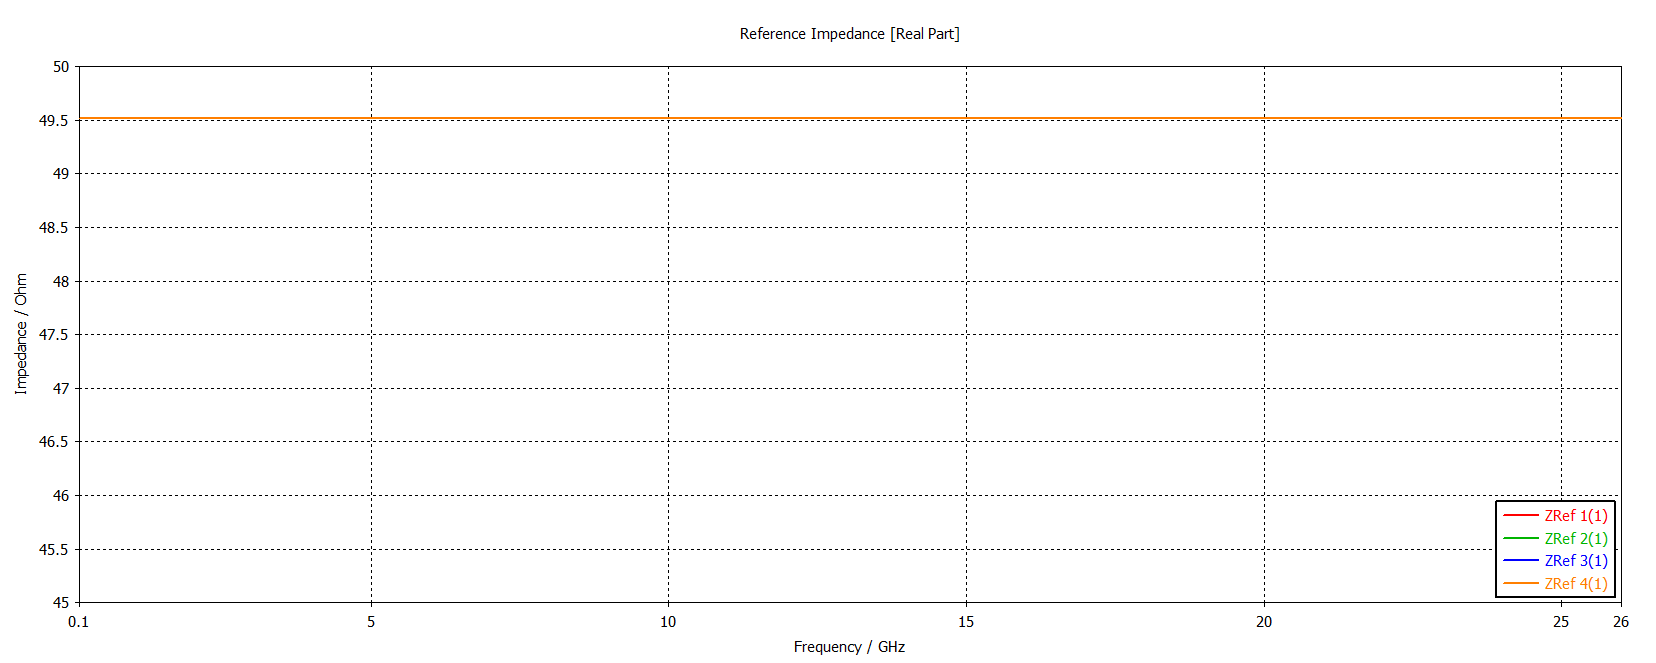
\includegraphics[width=.8\textwidth]{src/CST_Reference-Impedance_40dB_10-cpw_6-cntm.png}
	\end{figure}
\end{frame}

\section{Závěr}
\begin{frame}{Závěr}
	Cílem tohoto projektu bylo vyzkoušet si základní funkce softwaru CST Studio Suite pro modelování trojrozměrných struktur a jejich následnou elektromagnetickou analýzu.
    
    V rámci vypracování jsme se seznámili mimo jiné s různými parametry výpočtu, které mají výrazný dopad na přesnost řešení. Dopady perturbací jednotlivých parametrů na významné charakteristiky mikrovlnného obvodu byly ilustrovány na grafech, z nichž je možné posoudit významnost daného parametru ve výpočtu.

    Ze srovnání s průběhy S-parametrů vygenerovaných programem AWR Microwave Office specializovaným pro návrh mikrovlnných obvodů můžeme usoudit, že funkcionalita návrhu v programu CST dobře koreluje se zamýšlenou komponentou.
\end{frame}

\setbeamercolor{background canvas}{bg=white}

\end{document}
